% OCEANS 2027 abstract (submission limit: 2 pages, 500-1000 words incl. figures, equations and references; PDF).
% Status: draft started 2026-11-08 from paper/oceans2027_abstract_draft.md and
% paper/oceans2027_methods_results_draft.md; fact-checked against RESULTS_E7_SIM_DRYRUN.md the same day.
% Every result is from simulation (uwsim v0, uncalibrated) and is worded as such; the pool recordings
% (session S1 onward) replace or join them before submission.
% Build: python paper/fig_wer.py && latexmk -pdf -outdir=build oceans2027_abstract.tex   (run in paper/)
\documentclass[conference]{IEEEtran}
\usepackage[T1]{fontenc}
\usepackage{amsmath}
\usepackage{graphicx}
\usepackage{cite}
\usepackage{url}

\begin{document}

\title{Speech Enhancement versus Recognizer Adaptation for Underwater Speech Recognition over a Projector-to-Hydrophone Link}

% Sole author (lead's decision, 2026-11-19).
\author{\IEEEauthorblockN{Ryota Sato}
\IEEEauthorblockA{Department of Electrical Engineering, Stanford University\\
Stanford, CA, USA\\
\texttt{ryos17@stanford.edu}}}

\maketitle

\section{Motivation}
Divers, surface teams and underwater vehicles can exchange speech by driving an underwater projector
directly with audio-band speech (below 8~kHz, no carrier) and recording it with a hydrophone. The
speech arrives reverberant and mixed with thruster and bubble noise. Speech enhancement (SE) and
automatic speech recognition (ASR) models are trained on in-air audio. Through-water speech has been
simulated, recorded and enhanced before~\cite{nissen2017,roehrdanz2025,roehrdanz2026}, but those
recordings were not released, and to our knowledge no open benchmark measures SE or ASR on this
chain. The closest ASR work~\cite{rong2025} fine-tunes Whisper on in-mask speech and sends text over
an acoustic modem, so speech never crosses the water as audio. A vehicle that follows spoken commands
can either clean the audio before a frozen recognizer or adapt the recognizer itself. We compare the
two in simulation and are building a test-pool benchmark, with repeatable geometry and controlled
thruster noise, to compare them on recorded speech.

\section{Approach}
\textbf{Channel simulator.} \texttt{uwsim} models the path from a clean utterance $s$ to a hydrophone
recording as
\begin{equation}
y = Q\Big(\mathrm{HPF}\big(h_{\mathrm{hyd}} * \big(\textstyle\sum_{k=1}^{3} h_k * (\mathrm{LPF}_{8\,\mathrm{kHz}}\, s)^k * h_{\mathrm{ch}} + n\big)\big)\Big),
\end{equation}
where $(\cdot)^k$ is a pointwise power (third-order projector nonlinearity), $h_{\mathrm{ch}}$
combines image-source reflections, a stochastic late tail and a modal low band, $n$ is bubble or
stationary noise in the water, and $Q$ is a 24-bit converter. The results below use placeholder
parameters; calibrating them needs dedicated pool measurement takes, planned after the first session.

\textbf{Pool benchmark.} For the full paper, LibriSpeech test-clean utterances~\cite{panayotov2015}
are played in blocks of about 70~s framed by linear-FM sync chirps, at 1, 3 and 6~m, with the thruster
off and on in counterbalanced (off-on-on-off) order, and the first block repeated at the end to
check recorder drift. An import
pipeline, so far checked on synthetic recordings, aligns each recording to the playback schedule from
the chirps, corrects recorder clock drift and cuts every utterance. Each utterance's signal-to-noise
ratio (SNR) is estimated from its thruster-off recording and a separate noise-only recording.

\textbf{Systems.} Unprocessed audio; published enhancers used as is (weighted prediction error (WPE)
dereverberation, MetricGAN+, SepFormer and DeepFilterNet3~\cite{schroeter2023}); DeepFilterNet3 and a
U-Net trained on \texttt{uwsim}; and recognizer adaptation: Whisper large-v3~\cite{radford2023} with
low-rank adaptation (LoRA~\cite{hu2022}, rank~8) trained on simulated audio, with no front end and its
checkpoint chosen by WER on a separate simulated development set. Systems are compared by corpus word
error rate (WER) with paired speaker-cluster bootstrap 95\% confidence intervals (CIs), under an
evaluation protocol frozen before any pool recording is scored.

\section{Results so far (simulation)}
On 200 simulated test utterances from 40 speakers, enhancement did not carry over with range
(Fig.~\ref{fig:wer}). Fine-tuned DeepFilterNet3 lowered WER at 1~m in quiet ($-0.8$ points, CI
excluding zero) but raised it at 3 and 6~m ($+2.3$ and $+4.9$ points), and no front end lowered WER
in stationary noise by more than 0.1 points. Against the transducer-chain reference (the utterance
through the projector and hydrophone responses only, with no water path), the trained
enhancers raised extended short-time objective intelligibility (ESTOI)~\cite{jensen2016} at 6~m in
quiet from 0.36 to 0.56--0.61 while roughly doubling WER (4.3\% to 8.0--9.2\%). This agrees, in
simulation, with the in-air finding that enhancement artefacts hurt ASR~\cite{iwamoto2022}.

The adapted recognizer lowered WER in all 9 cells (quiet, bubble noise and stationary noise, each at
1, 3 and 6~m), significantly in 8; at bubble
noise and 1~m the drop (2.4\% to 2.2\%) was within the CI, near the 2.1\% of the transducer chain
alone. Under stationary noise at 0~dB SNR, with its spectral slope held out of training, WER fell from
20.3/48.4/56.4\% to 16.4/38.2/43.8\% at 1/3/6~m, a relative reduction of about 20\% at every range.
Unlike the enhancers, this adapter saw synthetic stationary noise at other spectral slopes in
training, so the stationary-noise comparison favors it.
A second seed, with its checkpoint chosen by validation loss, gave 16.0/37.2/44.5\%.

Under unconstrained beam search, one adapted model sometimes transcribed an utterance correctly and
then failed to stop, appending about 200 invented words (46 of 1200 quiet and bubble-noise decodes).
A decode-length cap tied to audio duration removed every such loop and moved unadapted WER by at most
0.1 points.

\begin{figure}[t]
\centering
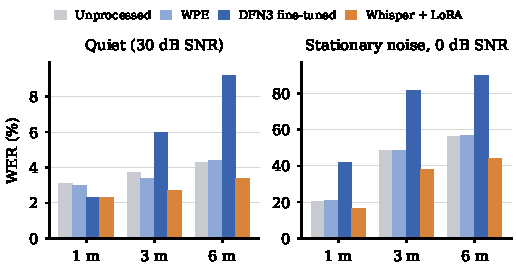
\includegraphics[width=\columnwidth]{fig_wer.pdf}
\caption{Whisper large-v3 WER on simulated hydrophone audio (\texttt{uwsim} v0, uncalibrated; no
pool recordings yet), in quiet and in stationary noise at 0~dB SNR: unprocessed audio, WPE (level with
unprocessed audio in every cell), DeepFilterNet3 fine-tuned on the simulator, and Whisper with LoRA.}
\label{fig:wer}
\end{figure}

\section{Contributions of the full paper}
\begin{itemize}
\item An openly released pool benchmark of projector-to-hydrophone speech, thruster off and on, with
aligned utterance cuts, per-utterance SNR and a frozen protocol.
\item A channel simulator, released with the paper and calibrated on pool measurements.
\item A comparison of enhancing the audio versus adapting the recognizer on simulated and recorded
speech, with a guard against run-on transcripts.
\end{itemize}

\begin{thebibliography}{1}
\bibitem{nissen2017} I.~Nissen and E.~Kuhnt-Matth\'e, ``Verbesserung der Sprachverst\"andlichkeit bei
analoger Unterwasserkommunikation durch Nutzung von digitalen Anfangs- und Endmarken,'' in
\emph{Proc. DAGA}, Kiel, 2017.
\bibitem{roehrdanz2025} F.~R\"ohrdanz \emph{et al.}, ``Data generation for training of neural networks
dealing with underwater speech transmission,'' in \emph{Proc. DAS|DAGA}, Copenhagen, 2025.
\bibitem{roehrdanz2026} F.~R\"ohrdanz \emph{et al.}, ``Neural-network based speech dereverberation for
underwater applications,'' in \emph{Proc. DAGA}, 2026, no.~144.
% TODO verify author initials and pages on IEEE Xplore (document 11104740).
\bibitem{rong2025} Y.~Rong \emph{et al.}, ``Underwater diver communication system based on speech/text
conversion,'' in \emph{Proc. OCEANS}, Brest, 2025.
\bibitem{panayotov2015} V.~Panayotov, G.~Chen, D.~Povey, and S.~Khudanpur, ``LibriSpeech: an ASR corpus
based on public domain audio books,'' in \emph{Proc. ICASSP}, 2015, pp.~5206--5210.
\bibitem{schroeter2023} H.~Schr\"oter, A.~N. Escalante-B., T.~Rosenkranz, and A.~Maier,
``DeepFilterNet: Perceptually motivated real-time speech enhancement,'' in \emph{Proc. Interspeech},
2023, pp.~2008--2009.
\bibitem{radford2023} A.~Radford \emph{et al.}, ``Robust speech recognition via large-scale weak supervision,'' in \emph{Proc. ICML}, 2023,
pp.~28492--28518.
\bibitem{hu2022} E.~J. Hu \emph{et al.}, ``LoRA: Low-rank adaptation of large language models,'' in
\emph{Proc. ICLR}, 2022.
\bibitem{jensen2016} J.~Jensen and C.~H. Taal, ``An algorithm for predicting the intelligibility of
speech masked by modulated noise maskers,'' \emph{IEEE/ACM Trans. Audio, Speech, Lang. Process.},
vol.~24, no.~11, pp.~2009--2022, 2016.
\bibitem{iwamoto2022} K.~Iwamoto \emph{et al.}, ``How bad are artifacts?: Analyzing the impact of speech enhancement errors on ASR,'' in
\emph{Proc. Interspeech}, 2022, pp.~5418--5422.
\end{thebibliography}

\end{document}
